\documentclass[uplatex]{jsarticle}

\usepackage{amsmath}
\usepackage[dvipdfmx]{graphicx}

\setcounter{tocdepth}{3}
\usepackage{float}
\usepackage{moreverb}
\usepackage{lscape}
\usepackage{url}
%\pagestyle{empty}
%\usepackage{wrapfig}
%\usepackage{url}
%\usepackage{EasyLayout}

\usepackage{ascmac}
%\usepackage{fancybx}

%\pagestyle{myheadings}


\begin{document}


\title{第8回目の課題}
\author{25G1065 塩澤匠生}
%\date{2015年11月13日}
\maketitle


\section{はじめに}
習志野市に10店舗を展開するCIT スーパーは売上高の減少に悩まされている.
そこで,この原因についての調査を行い,最も効率よく売上高減少を防止できる策を考える.


\section{手法}
調査のために,CITスーパーを統括するマネージャーは図\ref{fig:anket}に示すアンケートを作成し,実施した.
接客と品揃えと立地についての満足度を5段階で評価してもらいう形式で実施し,表\ref{table:anket_result}に示すような結果を得られた.
この結果から売上高と相関のある項目を見つけて,その項目を改善することで売上高の減少を防止することを目指す.



\begin{figure}[H]
    \centering
    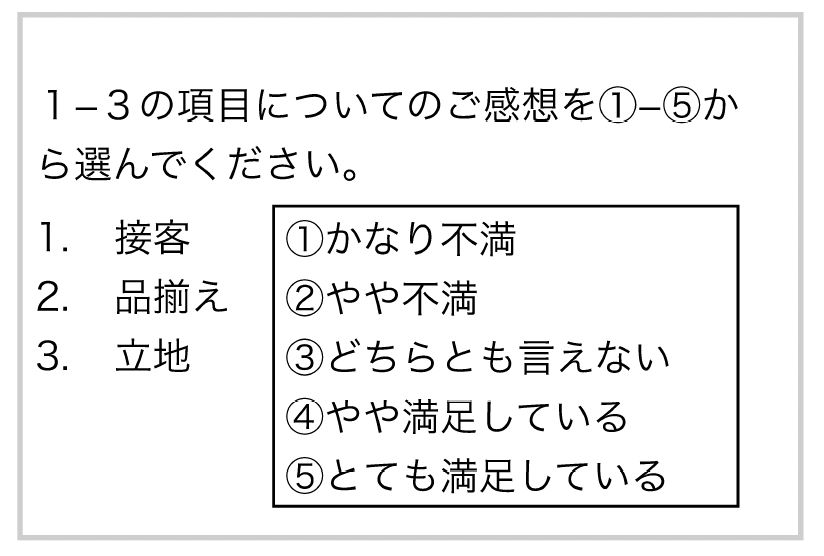
\includegraphics[width=0.5\textwidth]{anket.png}
    \caption{実施したアンケート}
    \label{fig:anket}
\end{figure}

\begin{table}[H]
    \centering
    \caption{実施したアンケートの結果}
    \label{table:anket_result}
    \begin{tabular}{ccccc}
        \hline
        店舗 & 1. 接客スコア & 2. 品揃えスコア & 3. 立地スコア & 売上高 (億円) \\\\ \hline
        A & 3.42 & 4.03 & 2.22 & 305.29 \\\\ \hline
        B & 4.49 & 4.07 & 1.84 & 281.99 \\\\ \hline
        C & 4.71 & 2.54 & 4.76 & 382.03 \\\\ \hline
        D & 0.39 & 3.11 & 3.62 & 346.11 \\\\ \hline
        E & 2.14 & 1.59 & 2.81 & 322.68 \\\\ \hline
        F & 4.67 & 4.63 & 1.63 & 277.73 \\\\ \hline
        G & 4.92 & 2.90 & 4.68 & 372.33 \\\\ \hline
        H & 4.13 & 2.85 & 2.69 & 314.68 \\\\ \hline
        I & 0.61 & 4.61 & 4.38 & 365.65 \\\\ \hline
        J & 3.78 & 3.10 & 4.28 & 357.50 \\\\ \hline
    \end{tabular}
\end{table}

\section{結果}
アンケートの結果をもとに,売上高と各スコアとの相関を調べた結果,図\ref{fig:correlation}に示すような結果が得られた.
各項目と売上高の相関係数を求めたところ,接客スコアとの相関係数は$r=-0.21$,品揃えスコアとの相関係数は$r=-0.37$,立地スコアとの相関係数は$r=0.99$となるということがわかった.
このことから,立地スコアが売上高に最も強い影響を与えていることがわかった.


\begin{figure}[H]
    \centering
    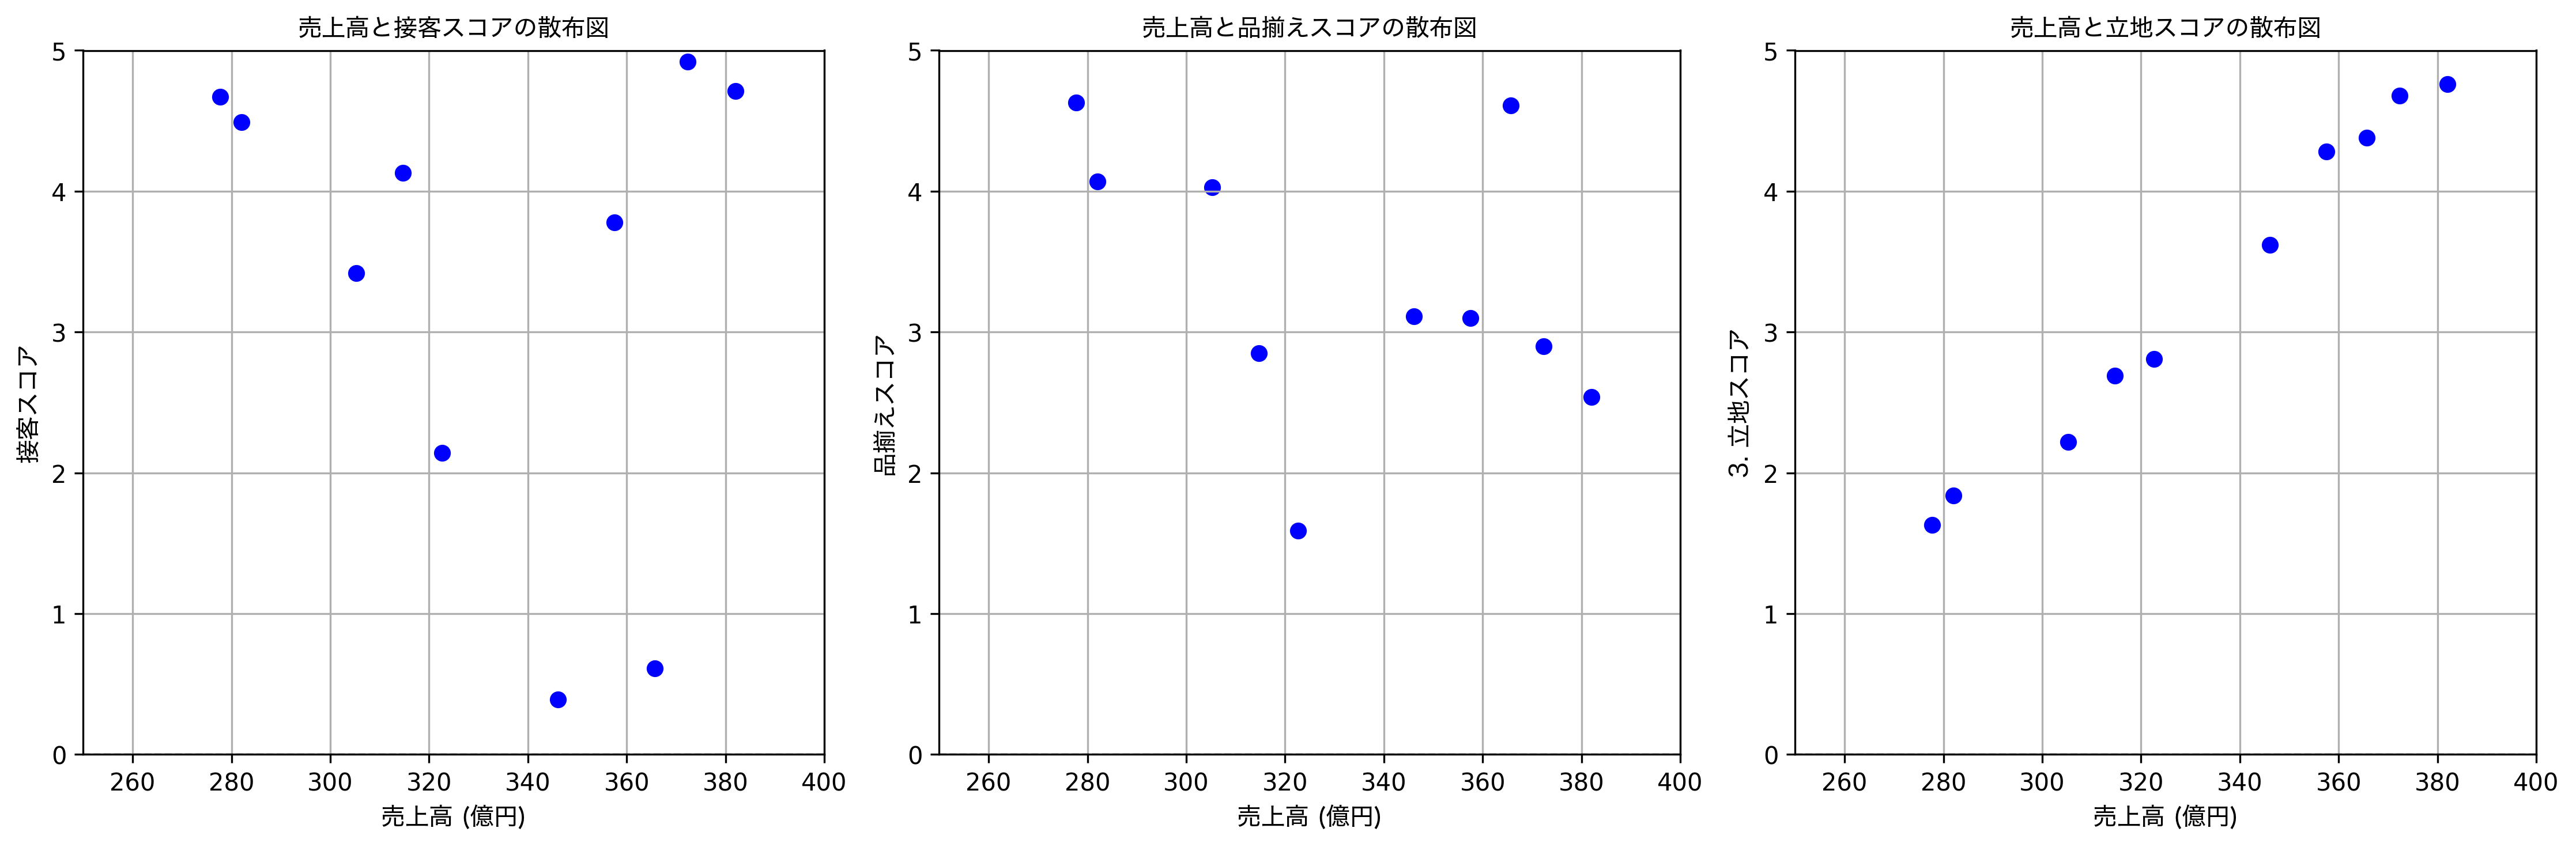
\includegraphics[width=1\textwidth]{graph/csv_graph.png}
    \caption{売上高と各項目の相関}
    \label{fig:correlation}
\end{figure}


\section{おわりに}


今回の調査はCITスーパーの売上高減少の原因を調べ,最も効率よく売上高減少を防止できる策を考えるために行われた.
その結果,今回の調査では立地スコアと売上高にに関する相関が最も高いということが明らかになった.

結果から,品揃えスコアと接客スコアと立地スコアの中では一番立地スコアが売上高に影響を与えていることがわかった.
そのため,次に出店する店舗を立地のいい場所にすることなどの立地に関する施策を行うことが最も効率よく売上高減少を防止できる策であると考えられる.

既存の研究との比較をしてみると,クロスロケーションズ株式会社の行ったコロナ禍におけるホームセンター/スーパーマーケット店舗の人流分析と売上動向の相関性についての調査によると,商品販売額と来訪数の相関係数は0.84と強い
相関が見られる\cite{crosslocations2021}ため,立地が良く人通りの多い場所に出店することが売上高減少を防止するために有効であると考えられる.

ただし,今回の調査ではあくまでも品揃えスコアと接客スコアと立地スコアの項目に関する調査しか行っていないため,
必ずしも立地のいい場所に出店することが最も効率よく売上高減少を防止できる策であるとは限らない.

今後の調査では他の項目に付いてのアンケートを行う必要があると考えられる.

これらの考察から,今回の調査では立地スコアが売上高に最も強い影響を与えていることがわかったので,
次に出店する店舗を立地のいい場所にするなど,立地に関する項目を改善した策を行うことが最も効率よく売上高減少を防止できると考えられる.


\begin{thebibliography}{9}
\bibitem{crosslocations2021} クロスロケーションズ株式会社, 【調査報告】コロナ禍におけるホームセンター/スーパーマーケット店舗の人流分析と売上動向の相関性についての調査レポート, クロスロケーションズ株式会社のプレスリリース, 2021.\url{https://moneyzone.jp/42040/?utm_source=chatgpt.com}
\end{thebibliography}
\end{document}



\end{document}



























